% gh d'après idée et premier td de Benoit Caritey
% 
% et http://static.ccm2.net/www.commentcamarche.net/contents/pdf/le-son-numerique-81-ljwlzc.pdf

\paragraph{Représentation informatique du son.}

Le son est une vibration de l'air, une suite de surpressions et de
dépressions de l'air. L'enregistrement d'un son, c'est
l'enregistrement de cette suite de variations de pression de l'air en
fonction du temps~: on parle de \emph{signal analogique}.

\centerline{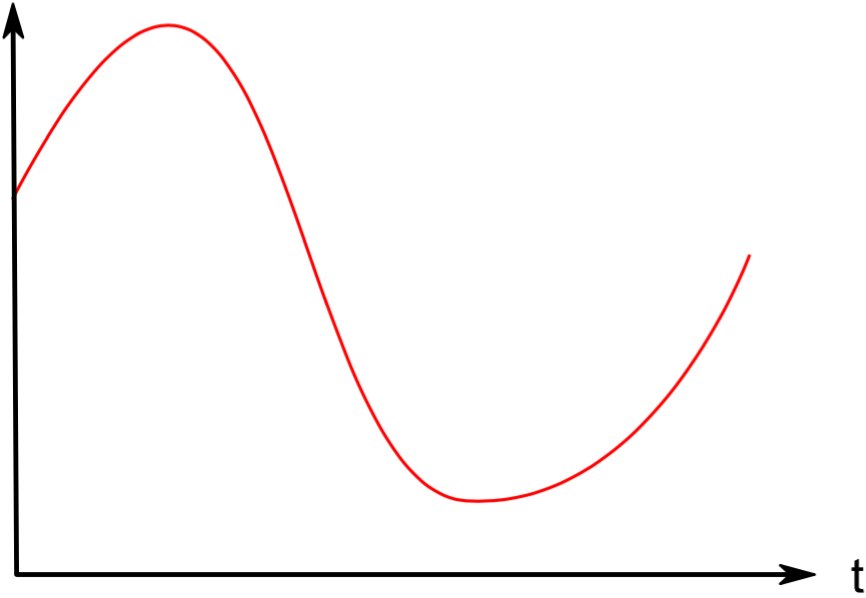
\includegraphics[height=3cm]{../input_exos_python/theme_son_2_fig_1}}

Pour représenter informatiquement un tel signal, on discrétise
l'information. On parle d'\emph{échantillonnage} ou de
\emph{numérisation}. Le \emph{signal numérique} est donc la suite des
valeurs du signal pour une succession d'instants bien définis. 

\centerline{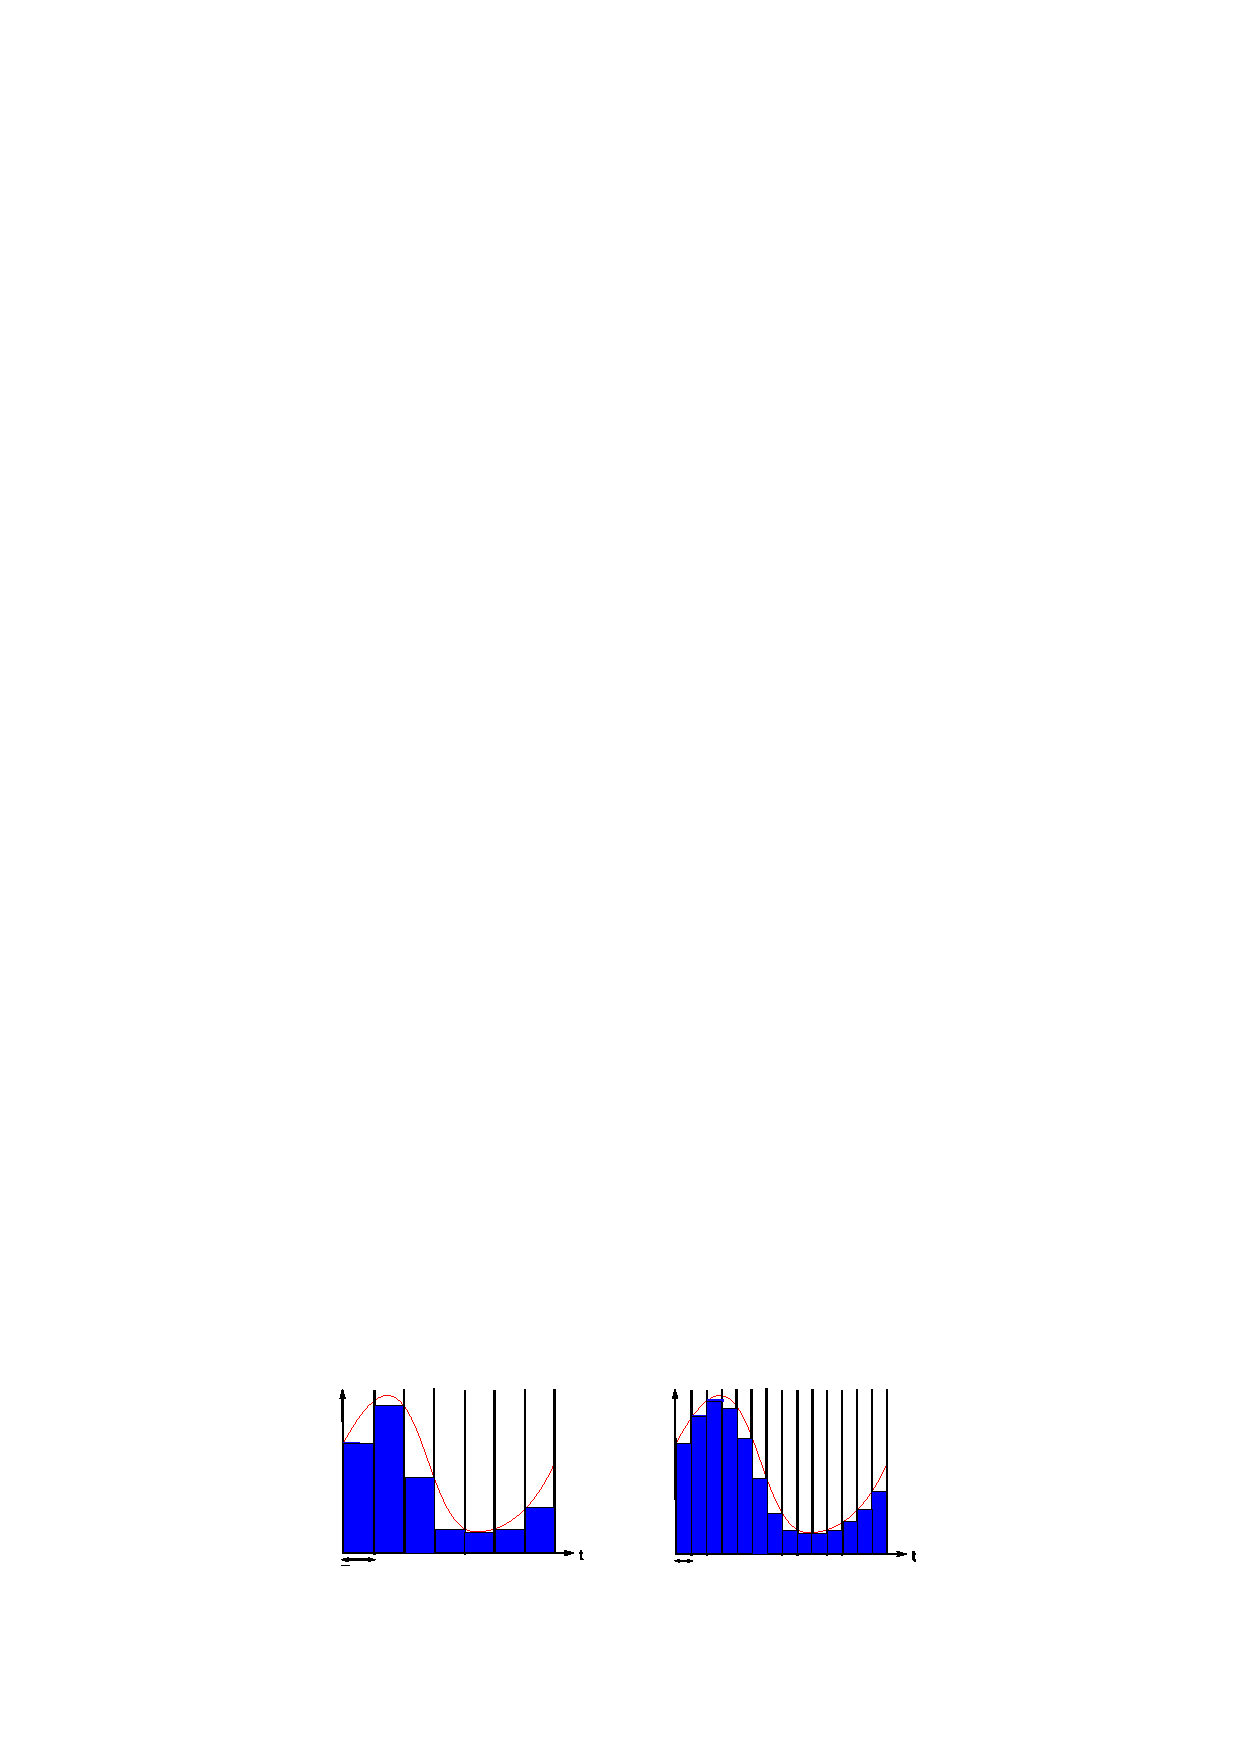
\includegraphics[height=3cm]{../input_exos_python/theme_son_2_fig_2}}

Lors de la numérisation, il y a une perte d'information plus ou moins
grande selon les valeurs choisies pour~: 
\begin{itemize}
\item 
  la \emph{fréquence d'échantillonnage} ou \emph{sample rate}. C'est le
  nombre de valeurs par seconde, exprimée en Hz. \\
  Le théorème de Shannon stipule que la fréquence d'échantillonnage doit
  être au moins le double de la fréquence maximale contenue dans le
  signal. Les fréquences les plus hautes (aiguës) perçues par l'oreille
  humaine sont de l'ordre de 20~kHz. \\
  On donne quelques valeurs courantes~: DVD~: 48~kHz, CD~: 44100~Hz,
  radio~: 22~kHz, téléphone~: 8~kHz  
  
\item 
  la \emph{résolution} ou \emph{bit depth}. C'est le nombre de bits
  servant à coder les valeurs à un instant donné. \\
  Avec 8 bits, seules 256 valeurs différentes sont utilisées, tandis
  qu'avec 16 bits, ce sont 65536 valeurs différentes qui sont
  utilisées, ce qui permet de représenter un son beaucoup plus riche. 
  \\
  On donne quelques valeurs courantes~: DVD~: 24~bits, CD~: 16~bits,
  téléphone et radio~: 8~bits 
\item 
  le \emph{nombre de voies} ou \emph{channel}. Il peut y en avoir 1 (mono), 2
  (stéréo), 6 (5.1) voire plus. 
\end{itemize}

\begin{enumerate}
\item 
  Quelle est la taille des données à stocker pour enregistrer
  10~minutes de musique sur un CD~? 
\end{enumerate}

% 10 minutes = 600 secondes donc 600*44100 valeurs
% chaque valeur est codée sur 16 bits soit 2 octets
% le son est en stéréo
% donc 600*44100*2*2 = 105 840 000 octets
% on divise par 1024 : 103 359 kO
% on divise encore par 1024 : 100,1 MO


\newpage

\paragraph{Manipulation de fichiers son avec Python}

Il existe de multiples normes, et de nombreux formats de fichiers pour
stocker des sons numérisés. Certains formats sont compressés, comme
\texttt{.mp3} ou \texttt{.aac}. D'autres ne sont pas compressés
comme \texttt{.wav} ou \texttt{.aif}. \\
Nous travaillons ici avec des fichiers \texttt{.wav}, que nous lirons
et écrirons grâce aux deux fonctions \verb#scipy.io.wavfile.read# et
\verb#scipy.io.wavfile.write#~:

\begin{python}
Help on function read in module scipy.io.wavfile:

read(filename, mmap=False)
    Return the sample rate (in samples/sec) and data from a WAV file    

    Parameters
    ----------
    filename : string or open file handle
        Input wav file.
    mmap : bool, optional
        Whether to read data as memory mapped.
        Only to be used on real files (Default: False)
    Returns
    -------
    rate : int
        Sample rate of wav file
    data : numpy array
        Data read from wav file    
    Notes
    -----    
    * The file can be an open file or a filename.
    * The returned sample rate is a Python integer
    * The data is returned as a numpy array with a
      data-type determined from the file.  
\end{python}

\begin{python}
Help on function write in module scipy.io.wavfile:

write(filename, rate, data)
    Write a numpy array as a WAV file
    
    Parameters
    ----------
    filename : string or open file handle
        Output wav file
    rate : int
        The sample rate (in samples/sec).
    data : ndarray
        A 1-D or 2-D numpy array of either integer or float data-type.    
    Notes
    -----
    * The file can be an open file or a filename.
    * Writes a simple uncompressed WAV file.
    * The bits-per-sample will be determined by the data-type.
    * To write multiple-channels, use a 2-D array of shape
      (Nsamples, Nchannels).  
\end{python}

La fréquence d'échantillonnage correspond donc à \verb#rate#.\\
La
résolution est donnée par le \verb#dtype# du tableau de données~: 
\verb#int8# ou \verb#int16#. \\
Le
nombre de voies est donné par le \verb#shape# du tableau de données~:
\verb#(n,)# ou \verb#(n,2)#. 

\newpage

\paragraph{Les questions}

\begin{enumerate}[resume*]
\item 
  Déterminer, pour les trois fichiers à télécharger sur le site de la
  classe, les caractéristiques du son (nombre de voies, fréquence,
  résolution). Préciser également la durée en secondes.  
\item 
  Définir une fonction \verb#affiche(filename)# qui affiche la
  première voie du signal sur un graphique. 
\item 
  Définir une fonction
  \verb#ajoute_silence(data, rate, duree_ms, debut=True)# 
  qui prend en arguments un tableau numpy de son mono, sa fréquence
  d'échantillonnage, la durée en ms du silence à ajouter, et un
  booléen indiquant si le silence doit être ajouté au début ou à la
  fin~; et qui renvoie le tableau numpy de son où un silence a été
  ajouté. 
\item 
  Définir une fonction
  \verb#mono_to_stereo(data, rate, duree_ms = 20)#
  qui prend en argument un tableau numpy de son, sa fréquence
  d'échantillonnage~; et renvoie un tableau numpy de son correspondant
  à deux voies identiques, mais la seconde sera décalée de 20 ms.
\item 
  Définir une fonction
  \verb#mixage(data, sound, rate, time, voie = 0)#
  qui prend en argument deux tableaux de son (l'un stéréo, l'autre
  mono), 
  la fréquence d'échantillonnage, un temps en secondes et le numéro
  d'une voie~; et renvoie un tableau numpy de son
  correspondant à \verb#data# où a été superposé \verb#sound# à partir
  de l'instant \verb#time#~s sur la voie~\verb#voie#. \\
  On ajoutera simplement les deux ondes sonores, sans se préoccuper de
  l'augmentation du gain et du risque de saturation. 
\item 
  Utiliser les fonctions précédentes pour créer un fichier stéréo,
  avec le bruit de la mer, un cri de mouette à gauche après 4
  secondes, un cri de mouette à droite après 12 secondes, puis, un peu
  plus tard, une sirène de bateau sur les deux voies. 

\item 
  Dégrader l'un des fichiers son pour qu'il soit au standard de la
  téléphonie. 
  % https://en.wikipedia.org/wiki/Decimation_(signal_processing)
\end{enumerate}

\vspace*{1cm}

\centerline{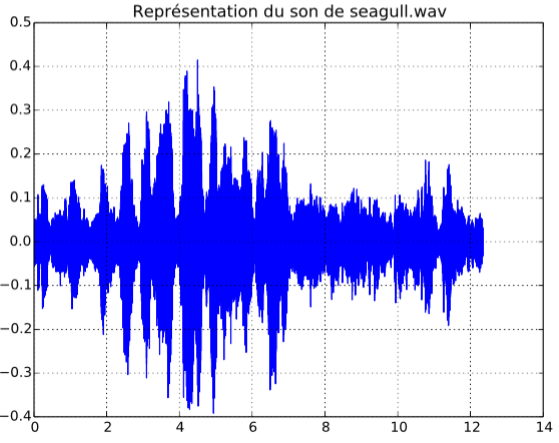
\includegraphics[width=.8\textwidth]{../input_exos_python/theme_son_2_fig_3}}
